\chapter[Introdução]{Introdução}

\section{Introdução}

Diante de problemas socioeconômicos, ambientais e geopolíticos relacionados ao uso do petróleo como principal fonte na matriz energética mundial, a busca por novas fontes de energia se faz necessária em todo mundo, e a utilização de recursos renováveis bem como o aproveitamento de resíduos sólidos descartados tem um importante papel no aproveitamento energético garantindo a diminuição dos impactos relacionados com uso de combustíveis fósseis. Nesse cenário, o Brasil tem grande destaque na produção de biocombustíveis, devido ao seu pioneirismo, se consolidou no mercado internacional com o etanol a partir da cana de açúcar \cite{santos2013bioenergia}.

O etanol, também denominado como álcool etílico ou apenas álcool, é um composto orgânico e foi um dos primeiros compostos químicos a ser preparado e purificado. Sua utilização se dá principalmente em bebidas alcoólicas, combustíveis e antissépticos \cite{de2004introduccao}. Ele é obtido desde tempos antigos a partir da fermentação de açúcares presente em grãos, vegetais, beterraba, cana-de-açúcar, mandioca, milho e trigo \cite{santos2013bioenergia}.

A fermentação alcoólica é um processo químico em que microrganismos metabolizam, por meio de suas enzimas, um substrato orgânico, o açúcar, e formam como principal produto o álcool \cite{furlan2009produccao}. Na indústria, o microrganismo mais empregado nesse processo é a levedura do tipo Saccharomyces cerevisiae, um fungo capaz de sobreviver em condições aeróbicas e anaeróbicas e que promove rendimentos altos na conversão de açúcar à álcool \cite{lima2001biotecnologia}.

\section{Objetivos}

\subsection{Objetivo Geral}

Esse trabalho tem por objetivo projetar e construir um biorreator automatizado para fermentação alcoólica, monitorando, via sensores, parâmetros de temperatura e pH durante o processo fermentativo.

\subsection{Objetivos Específicos}

\begin{itemize}
	\item Dimensionar e construir a estrutura do biorreator;
	\item Monitorar e regular a temperatura durante a fermentação, por meio de um sistema de aquecimento e resfriamento;
	\item Monitorar o pH durante a fermentação;
	\item Monitorar o teor de açúcar consumido durante a fermentação;
	\item Monitorar o aumento do teor alcoólico durante a fermentação;
	\item Capturar o CO2 produzido durante do processo de fermentação;
	\item Fazer o controle remoto dos parâmetros da fermentação;
	\item Criar plataforma para apresentação de dados referentes aos parâmetros analisados na fermentação.
\end{itemize}

\subsection{Problemática}

O crescimento das indústrias sucroalcooleiras se faz necessário diante aos impactos negativos causados ao meio ambiente com a utilização de combustíveis fósseis. Tendo este problema em vista, um dos maiores fatores concernentes à contínua utilização de combustíveis fósseis em maior escala no mundo é por causa de sua grande produção em escala devido à consolidação da indústria petrolífera e também por ser um recurso que se encontra em fase de processo automatizado e totalmente controlado. No Brasil, por exemplo, aproximadamente 35\%da energia primária consumida tem sua origem do Petróleo \cite{lucchesi1998petroleo}.

Para que se tenha um aumento na utilização de biocombustíveis, por consequência um aumento na indústria sucroalcooleira, para produção de etanol, os processos devem seguir uma linha mais direta e automatizada, como na indústria petrolífera. Esta automação do processo está intimamente ligada à diminuição de custos e de problemas no processo de obtenção do produto. Para que se obtenha o etanol é necessário o uso de biorreatores que são capazes de agitar a mistura durante o processo de fermentação alcoólica, e para que se tenha uma otimização dos parâmetros, algumas variáveis do processo precisam ser controladas.

A indústria do etanol possui grandes fermentadores e atualmente trabalham em grande escala, porém, focam sua automação na etapa de destilação. A necessidade da expansão de infraestrutura de produção para outras áreas de processos é uma das principais problemáticas enfrentadas neste processo \cite{lopes2008etanol}. Desta forma, na síntese de um biocombustível que necessita de fermentação em um biorreator, é necessário que alguns fatores sejam controlados para que o processo seja conduzido da melhor forma possível e que se obtenha uma produção máxima de recursos e produtos \cite{ribeiro2015fermentaccao}.

No Brasil, os grandes reatores possuem problemas devido a grande perda de eficiência na etapa de fermentação. Essa perda se deve à alguns fatores como:

\begin{itemize}
	\item Falta de refrigeração no processo;
	\item Perda de grau alcóolico por falta de introdução de açúcares durante a operação;
	\item Reativação dos microrganismos para estabilidade operacional;
	\item Falta de monitoramento de parâmetros com sensores específicos;
	\item Processo com falta de automação.
\end{itemize}

Desta forma, a construção de reatores automatizados e capazes de controlar o processo evitaria a perda de eficiência durante a fermentação. Neste caso, os principais parâmetros de um reator e que precisam ser controlados são: pH, temperatura, densidade, espuma, níveis de reservatório, agitação, portas de amostragem e sistema de limpeza. Assim, uma produção inteiramente automatizada e baseada em inovações tecnológicas garante uma maior eficiência do processo além de eliminar os problemas relacionados ao controle dos parâmetros de forma manual, diminuindo assim os custos de integração e produção de produtos finais.

Os problemas citados acima juntamente com as respectivas causas e efeitos da problemática abordada pelo grupo está exemplificado no diagrama de fishbone abaixo, \ref{fishbone}.

\begin{figure}[h]
	\centering
	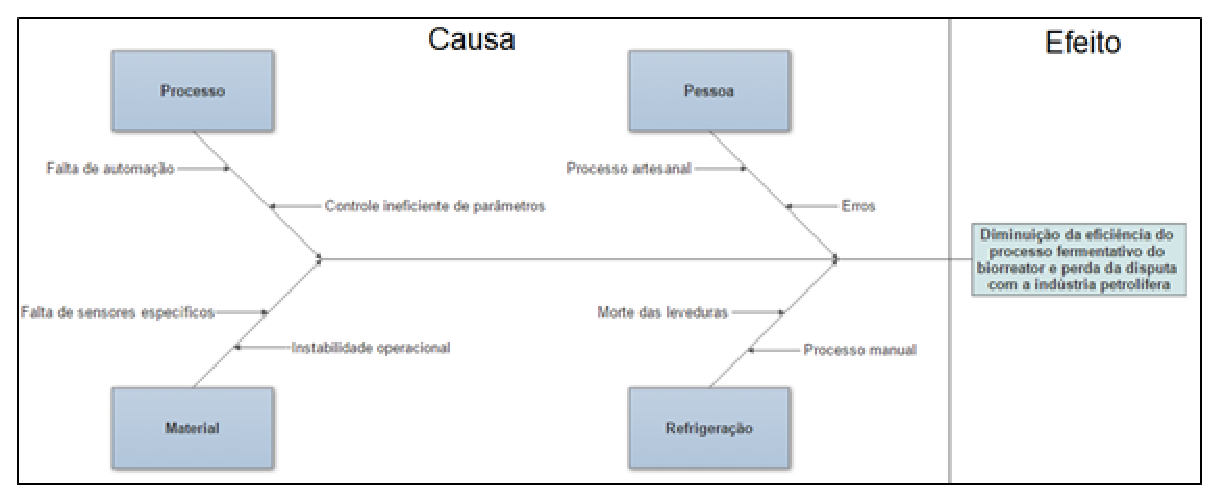
\includegraphics[keepaspectratio=true,scale=0.8]{figuras/fishbone.eps}
	\caption{Fishbone do Mapeamento do Problema}
	\label{fishbone}
\end{figure}

Para uma melhor descrição do problema, um pré-escopo do problema apresentado abaixo, descreve de forma mais formal o problema a ser solucionado pelo grupo:

\textbf{Problema:} Falta de automação e controle de parâmetros de um biorreator.

\textbf{Efeito:} Perda de eficiência do processo devido a instabilidade operacional.

\textbf{Solução:} Construção de um biorreator automatizado capaz de controlar parâmetros importantes como pH, temperatura, agitação e densidade durante o processo, possuindo uma interface com o usuário.

\subsection{Jusificativa}

A \textit{Saccharomyces cerevisiae} é um microrganismo sensível, que é diretamente influenciada pelo meio em que está, de forma que todos os parâmetros da fermentação devem ser ajustados e monitorados para que ela tenha o seu melhor desempenho, além disso, essa regulação do meio evita a contaminação ou a perda dessas leveduras, que estão relacionadas de forma direta à qualidade do álcool produzido.

Tendo isso em vista, a construção de um biorreator automatizado se faz justificada, uma vez que haverá o monitoramento constante de todos os parâmetros que influenciam a qualidade e o desenvolvimento das leveduras. Além disso, levando em conta a importância do Brasil na produção mundial de etanol e a necessidade de novas biomassas para produção de biocombustíveis, esse biorreator se mostra relevante para ser utilizado em pesquisas acadêmicas, uma vez que a fermentação é a etapa mais importante de produção do álcool.

\subsection{Estado da arte}

A produção de biocombustíveis é uma das premissas de desenvolvimento sustentável que mais cresce no mundo, devido, principalmente, a descarga de gases poluentes com a utilização de combustíveis fósseis. Tendo isto em vista, a produção de etanol, um dos principais biocombustíveis do Brasil deverá aumentar, junto a isso, a pesquisa conjunta em Universidades de todos os países sobre este tipo de assunto deverá aumentar também. Segundo \cite{leite2007biocombustivel}, a produção de biocombustíveis, a princípio o etanol, aumentará cerca de 50\% nos próximos 20 anos. Desta forma, estudos de viabilidades de produção serão necessários para este crescimento assim como equipamentos capazes de otimizar o processo de obtenção destes biocombustíveis.

O biorreator, também chamado de fermentador, é um dos equipamentos capazes de produzir diversos tipos de misturas, uma delas o biocombustível, porém, biorreatores de bancadas são quase sempre feitos de modo rústico e manuseados apenas por instrumentação individual, colocando assim, a eficiência do projeto em risco. Para um melhor estudo, um biorreator automatizado e capaz de controlar os parâmetros das reações seria necessário, mas por motivos de aplicação industrial, hoje os fermentadores deste tipo custam acima de R\$ 10.000,00 e seus modelos ultrapassam 30 litros de capacidade, o que inviabiliza os estudos em bancada, um exemplo de um biorreator automatizado encontrado em mercados está exemplificado na Figura \ref{tecnopon}, da marca Tecnopon, com capacidade de 150 L e sensores de pH, O2, temperatura além de possuir motor de agitação, comunicação com o usuários via transmissor e bomba de circulação de água refrigeradora interna e aquecimento por resistência interna, seu preço de mercado é de aproximadamente R\$ 15.000,00.

\begin{figure}[h]
	\centering
	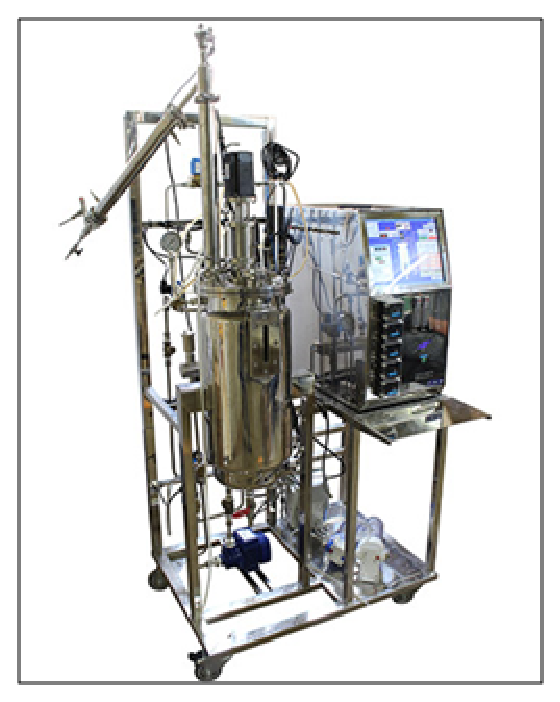
\includegraphics[keepaspectratio=true,scale=0.8]{figuras/tecnopon.eps}
	\caption{Biorreator industrial com capacidade de 150 L da marca Tecnopon}
	\label{tecnopon}
\end{figure}

Biorreatores mais simples também são construídos devidos ao aumento de produção de cerveja artesanal e existem diversas opções de biorreatores para fermentação alcoólica disponíveis no mercado, variando em volume, material e formato. Apesar de diversas empresas trabalharem com o fermentador personalizado de acordo com a necessidade de cada cliente, não foi encontrado biorreatores de forma automatizada, o mais próximo foi um fermentador da marca Basinox, mostrado na Figura \ref{basinox}, que faz apenas controle digital de temperatura.

\begin{figure}[h]
	\centering
	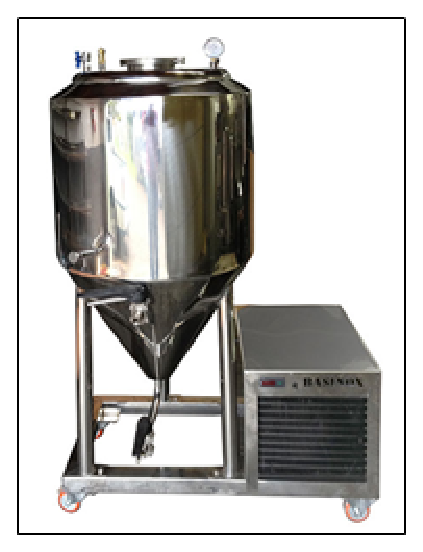
\includegraphics[keepaspectratio=true,scale=0.8]{figuras/basinox.eps}
	\caption{Fermentador da marca Basinox}
	\label{basinox}
\end{figure}

Outra opção utilizada, principalmente para produção de cerveja
artesanal, é a venda do \textit{Ardbir}, um equipamento que faz controle PID da
temperatura. Porém, apesar dele poder ser utilizado como forma de controle na
fermentação, ele é mais utilizado na etapa de preparação do mosto, que demanda
diversas variações de temperatura em longos períodos de tempo.

Desta forma, busca-se neste trabalho, a construção de biorreator de bancada capaz de apresentar algumas dessas características desses biorreatores mais desenvolvidos industrialmente, levando em consideração a condição acadêmica de pesquisa e seu baixo custo.

\subsection{Escopo}

Após a análise da problemática realizada pelo grupo, foram estipuladas as medidas que seriam realizadas, definindo-se assim o escopo geral do projeto. Dessa forma, foi decidido que para fins de protótipos, o biorreator terá as seguintes características:

\begin{itemize}
\item Capacidade de medir pH do meio;
\item Capacidade de monitorar e regular, se necessário, a temperatura do meio por controle PID;
\item Capacidade de medir a variação de densidade por meio da diferença de pressão do mosto;
\item Sistema para tratar dados referentes a variação de densidade, fazendo a  conversão para ºBrix e teor alcoólico;
\item Capacidade de gerar curvas relacionadas ao aumento do teor alcoólico pelo consumo do açúcar no meio;
\item Capacidade de realizar o controle de tais parâmetros de forma remota via aplicativo;
\item Capacidade de coletar o CO2 produzido durante o processo de fermentação alcoólica.
\end{itemize}

É importante ressaltar, que esse projeto abrange apenas a parte de fermentação, que é apenas uma das etapas na produção do álcool. Dessa forma, é possível produzir diversos fermentados, como etanol combustível, cerveja e vinho, variando apenas no preparo do mosto anterior ao processo de fermentação e concluindo com etapas seguintes à fermentação, como destilação para o caso do etanol e carbonatação e engarrafamento para cerveja.
